\begin{figure}[htp]
	\centering
	\subfloat[\(\Re{\pixel{(\translation{\omega'}f_{A})}}\)]{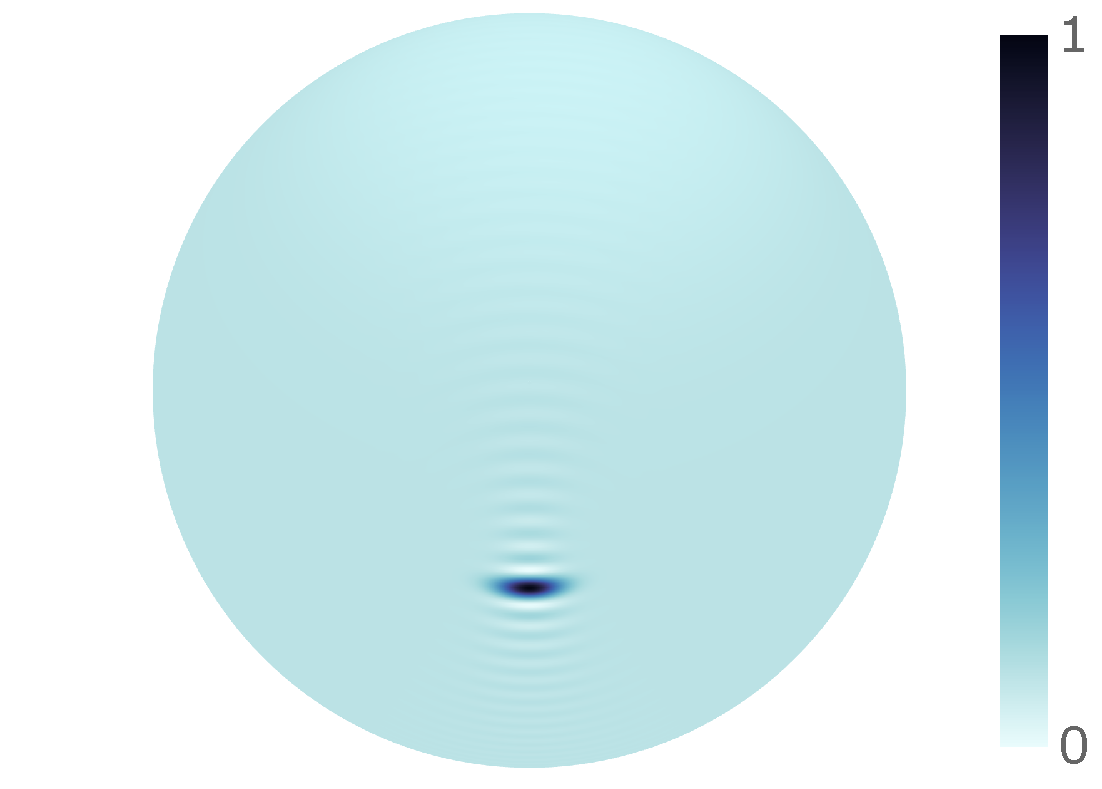
\includegraphics[trim={22 9 7 6},clip,width=.5\textwidth]{harmonic_gaussian_100lsig_10msig_L128_translate_alpha3pi4_beta1pi8_res512_real_norm.pdf}}
	\hfill
	\subfloat[\(\Re{\pixel{(\translation{\omega'}f_{B})}}\)]{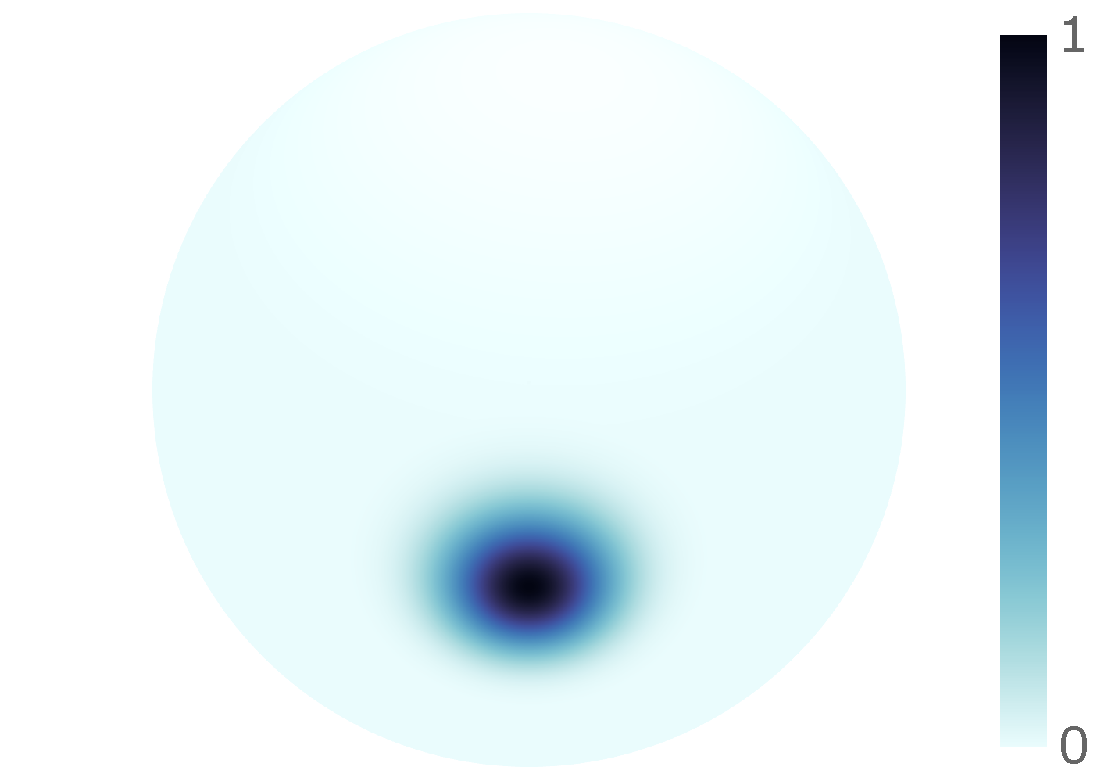
\includegraphics[trim={22 9 7 6},clip,width=.5\textwidth]{harmonic_gaussian_10lsig_10msig_L128_translate_alpha3pi4_beta1pi8_res512_real_norm.pdf}}
	\caption{
		A harmonic Gaussian translated to some \(\omega'=(\theta',\phi')\) (bandlimited at \(L=128\)).
		Panel (a) corresponds to a more elongated kernel \(f_{A}\), where \((\sigma_{\ell},\sigma_{m}) = (10^{2}, 10^{1})\); whereas panel (b) corresponds to a more symmetric kernel \(f_{B}\), where \((\sigma_{\ell},\sigma_{m}) = (10^{1}, 10^{1})\).
		The colour is between zero and one, reflecting the scaled intensity of the field.
	}\label{fig:chapter2_translated}
\end{figure}
